\section{1174040 - Hagan Rowlenstino A. S}
    \subsection{Teori}
    \begin{enumerate}
        \item Kenapa file suara harus dilakukan MFCC
        \subitem MFCC digunakan untuk mengidentifikasi jenis suara yang dimasukan seperti suara lagu, hujan atau pun suara yang tidak dapat didengar oleh telinga manusia yaitu Ultrasonik, sehingga dibutuhkan penggunaan MFCC untuk memproses data tersebut agar dapat dibaca oleh manusia. ilustrasi untuk MFCC dapat dilihat pada gambar
        
        \begin{figure}[H]
            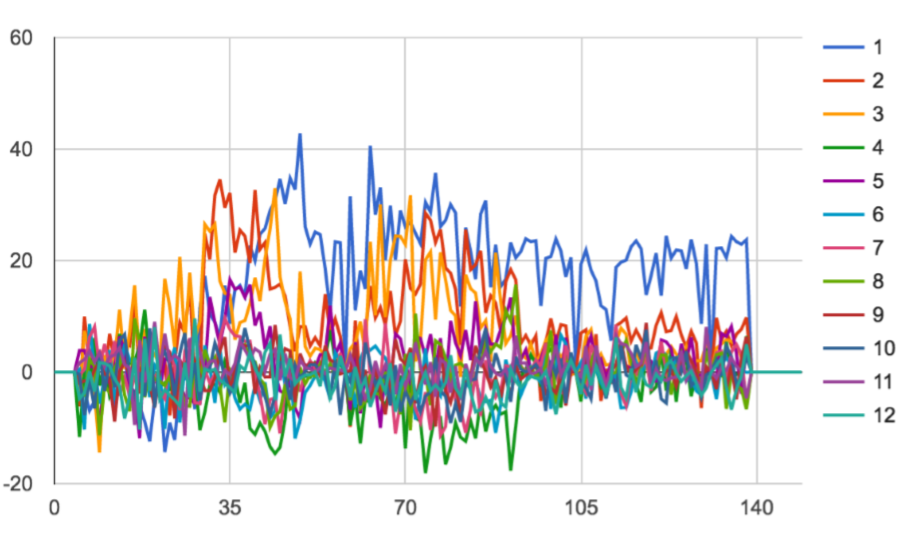
\includegraphics[width=4cm]{figures/1174040/chapter6/teori1.png}
            \centering
              \caption{Ilustrasi MFCC}
        \end{figure}
        
        \item Konsep dasar Neural Network
        \subitem Neural Network sebenarnya mengadopsi dari kemampuan otak manusia yang mampu memberikan stimulasi/rangsangan, melakukan proses, dan memberikan output. Output diperoleh dari variasi stimulasi dan proses yang terjadi di dalam otak manusia.
        ilustrasi Neural Network dapat dilihat pada gambar
        
        \begin{figure}[H]
            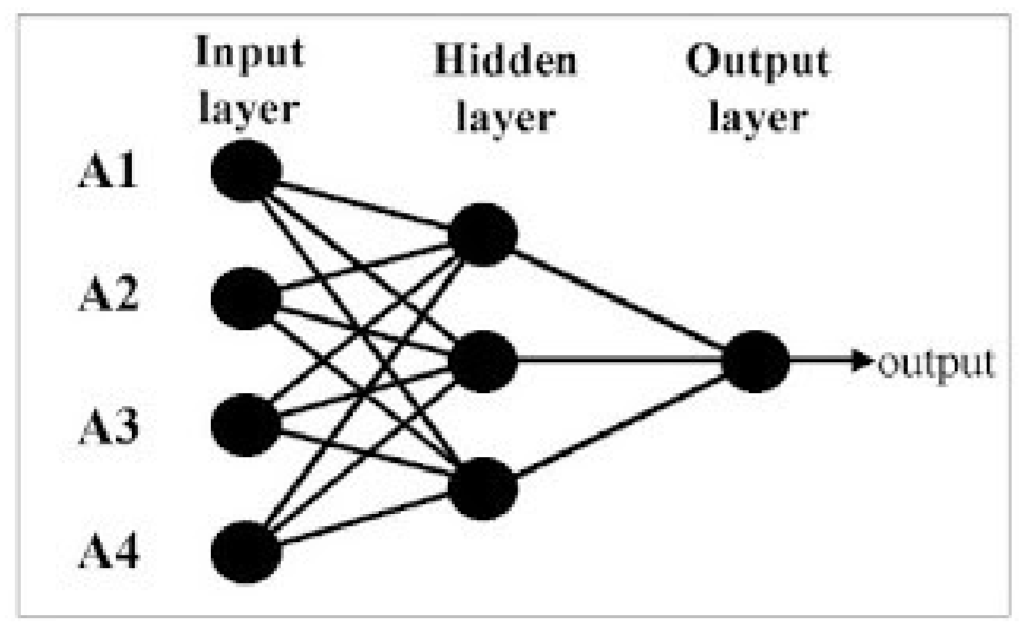
\includegraphics[width=4cm]{figures/1174040/chapter6/teori2.png}
            \centering
              \caption{Ilustrasi Neural Network}
        \end{figure}
        
        \item Konsep Pembobotan dalam Neural Network
        \subitem konsep pembobotan dalam neural network digunakan untuk membedakan data satu dengan data lainnya, sebagai contoh dapat dilihat pada gambar. dimana data inputan yang masuk adalah 2 data yaitu "anjing" dan "kucing" yang diolah dengan proses membandingkan data dan diolah melalui pembobotan sehingga menampilkan hasil output.
        
        \begin{figure}[H]
            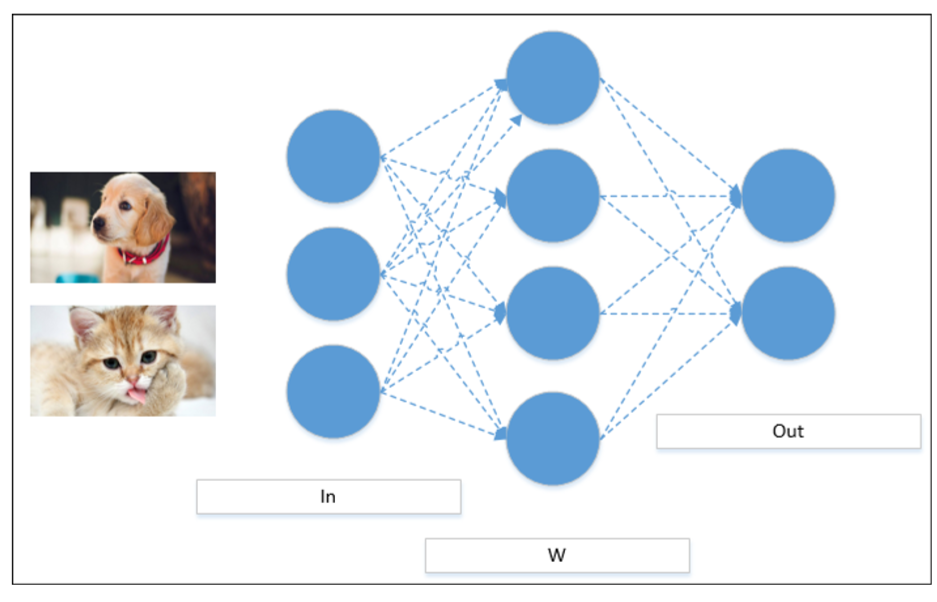
\includegraphics[width=4cm]{figures/1174040/chapter6/teori3.png}
            \centering
              \caption{Ilustrasi pembobotan Neural Network}
              
        \end{figure}
        
        \item Konsep Aktifasi dalam Neural Network
        \subitem dalam Neural Network fungsi aktifasi meliputi inputan dan diproses sehingga menghasilkan Output nilai yang diharapkan, dengan menggunakan persepsi alur cara penyampaian informasi pada jaringan syaraf otak. ilustrasi dapat dilihat pada gambar
        
        \begin{figure}[H]
            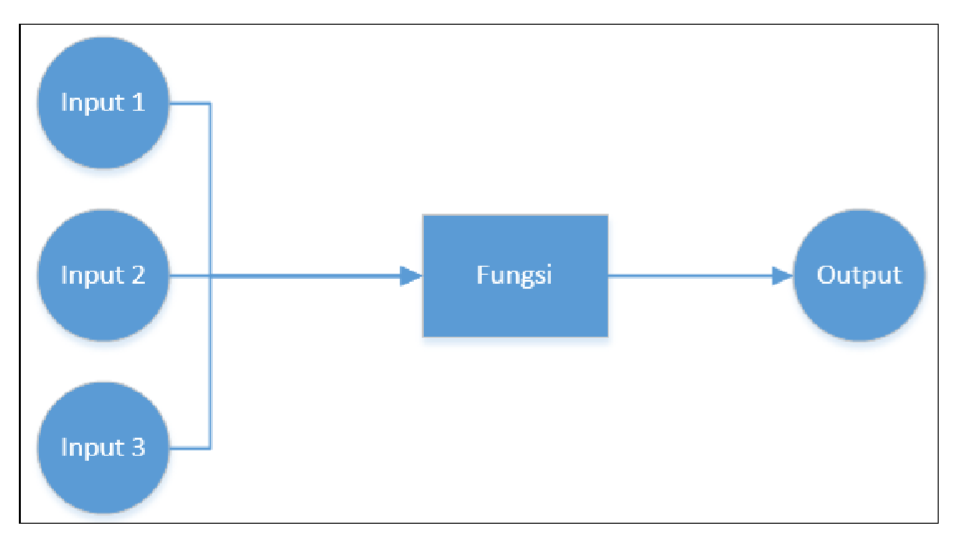
\includegraphics[width=4cm]{figures/1174040/chapter6/teori4.png}
            \centering
              \caption{Ilustrasi fungsi aktifasi Neural Network}
              \label{f4}
        \end{figure}
        
        \item cara membaca hasil PLOT dari MFCC
        
        \begin{figure}[H]
            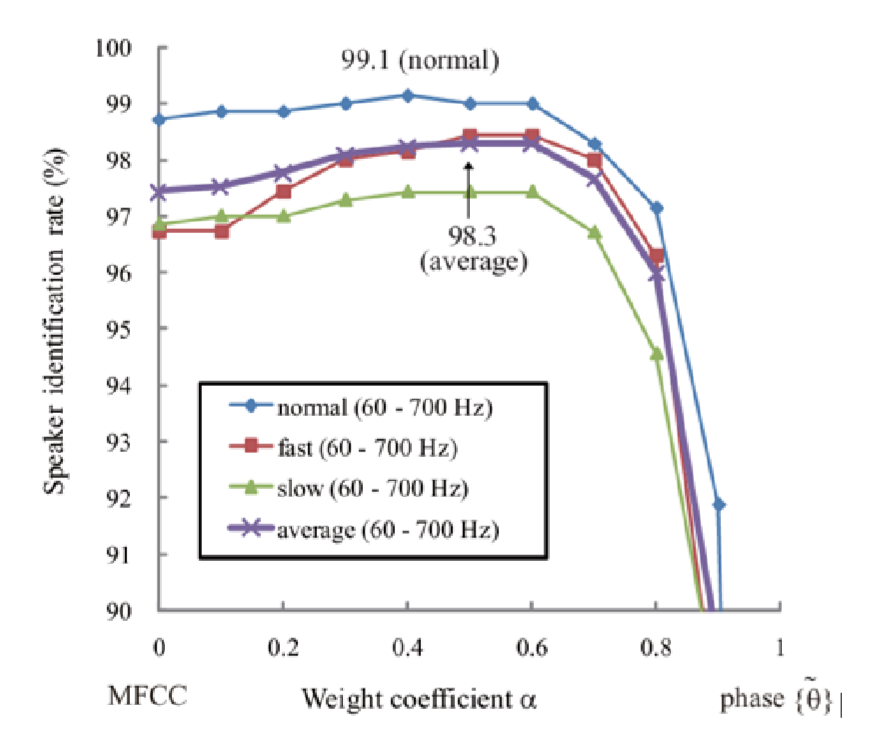
\includegraphics[width=4cm]{figures/1174040/chapter6/teori5.png}
            \centering
              \caption{Ilustrasi Membaca nilai Plot dari MFCC}
        \end{figure}
        
        \item One-hot Encoding
        \subitem penggunaan One-hot Encoding adalah dengan membaca data yang memiliki nilai 1 sebagai nilai tinggi atau bisa disebut juga sebagai nilai positif dan 0 sebagai nilai rendah yang bermakna juga sebagai nilai negatif. ilustrasi dapat dilihat pada gambar

        \begin{figure}[H]
            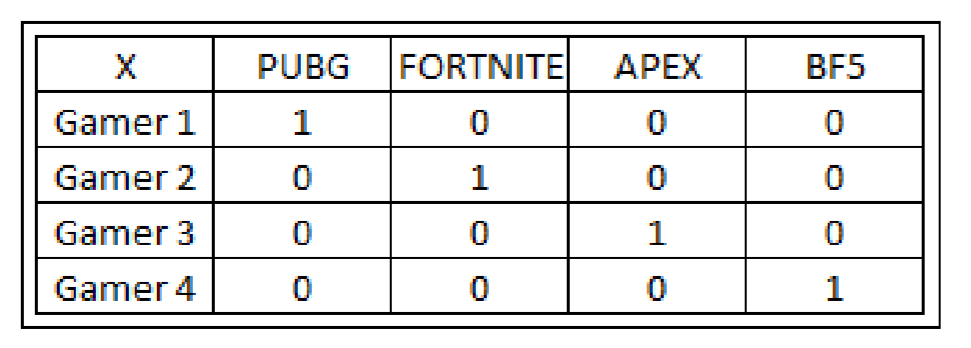
\includegraphics[width=4cm]{figures/1174040/chapter6/teori6.png}
            \centering
              \caption{Ilustrasi One-hot Encoding}
        \end{figure}
        
        \item fungsi dari np.unique dan to\_categorial dalam Code Program
        \subitem fungsi dari NP.UNIQUE dalah untuk membuat data elemen menjadi nilai yang bersifat unik dalam artian (Array), ilustrasi dapat dilihat pada gambar
        
        \begin{figure}[H]
            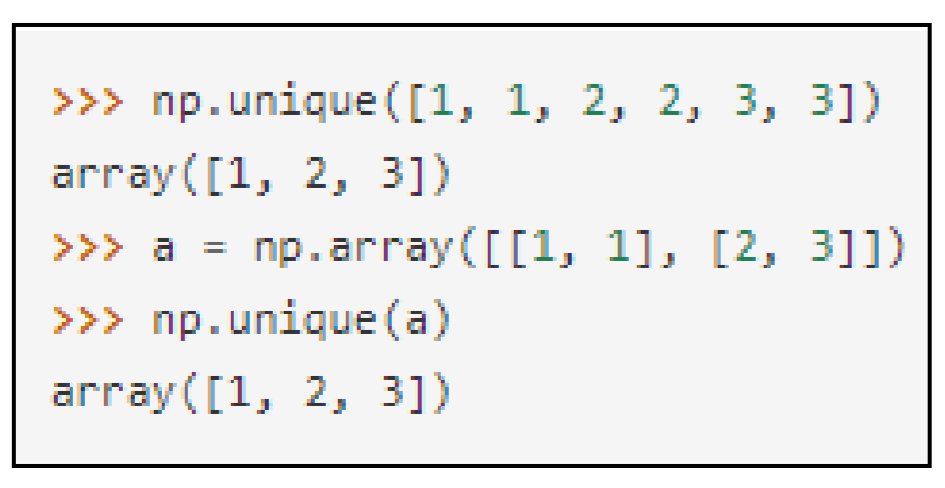
\includegraphics[width=4cm]{figures/1174040/chapter6/teori7.png}
            \centering
              \caption{Ilustrasi np.unique}
        \end{figure}
        
        \subitem sedangkan perintah to\_categorial adalah untuk membuat data integer yang terdeteksi untuk diubah menjadi data matrix biner. ilustrasi dapat dilihat pada gambar
        
        \begin{figure}[H]
            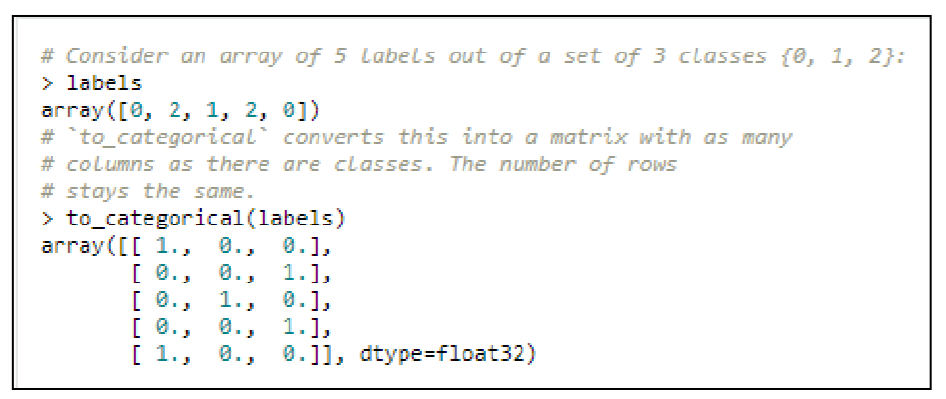
\includegraphics[width=4cm]{figures/1174040/chapter6/teori8.png}
            \centering
              \caption{Ilustrasi to\_categorial}
        \end{figure}
        
        \item fungsi dari Sequential
        \subitem fungsi dari Sequential dari code program adalah untuk membagi data - data agar dapat dianalisis oleh sistem lebih mudah, misalkan dari data 100 dibagi prosesnya menjadi 4 yaitu 25 perproses, seperti yang terdapat pada gambar \ref{f9} sehingga hasil yang didapatkan akan lebih baik lagi.
        
        \begin{figure}[H]
            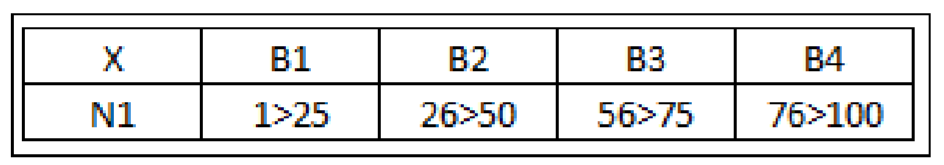
\includegraphics[width=4cm]{figures/1174040/chapter6/teori9.png}
            \centering
              \caption{Ilustrasi fungsi Sequential}
        \end{figure}
        \end{enumerate}

    \subsection{Praktek}
        \begin{enumerate}
            \item Penjelasan data GTZAN Genre Collection dan Freesound, Buat Code Program untuk Load data Tersebut.
            \subitem GTZAN Genre Collection merupakan datasets yang berisi data lagu yang terdiri dari 10 genre yaitu :
            \begin{itemize}
            \item Blues
            \item Classical
            \item Country
            \item Disco
            \item Hip-Hop
            \item Jazz
            \item Metal
            \item Pop
            \item Reggae
            \item Rock
            \end{itemize}
            10 genre tersebut memiliki data sebesar 100 data suara.
            
            \subitem sedangkan Freesound merupakan sebuah contoh suara yang digunakan untuk menguji hasil dari pengolahannya dengan menggunakan metode MFCC, untuk mencari genre yang pas bagi contoh suara tersebut.
            
            \lstinputlisting[firstline=1, lastline=10]{src/1174040/chapter6/1174040.py}
            
            \subitem Code tersebut digunakan untuk memanggil library Librosa yang memuat metode Feature dan Display yang akan digunakan untuk memproses data suara tersebut dengan MFCC. lalu Library Glob yang digunakan untuk mencocokan pattern yang spesifik dari data tersebut, Library Numpe yang digunakan untuk membuat data Vector, Library matplotlib yang digunakan untuk membuat data grafik dan Library Keras adalah open-source yang bekerja untuk memproses TensorFlow, CNTK dan Theano, yang didesain untuk melakukan penelitian dengan menggunakan Deep Neural Network.
            
            \item Penjelasan Code Program display\_mfcc
            
            \lstinputlisting[firstline=12, lastline=22]{src/1174040/chapter6/1174040.py}
            
            \subitem Code tersebut meliputi penggunaan MFCC dengan proses Display yang memiliki penjelasan seabgai berikut, Variable Y berisi Library Librosa dengan method LOAD dan berisi nilai SONG sebagai penggunaan classnya. dan Variable MFCC yang berisi method feature.mfcc dan memiliki nilai dari Variable Y. penggunaan plt sebagai pemanggilan matplotlib dengan method FIGURE yang akan menampilkan data gambar. dan Librosa yang akan menampilkan method display.specshow dengan data dari Variable mfcc dan pengaturan Axis X dan Y. lalu mengisikan data dengan nilai dari COLORBAR, TITLE yang berisi data dari class SONG dan tight\_layout serta show yang akan menampilkan hasil RUN yang dilakukan.
            
            \subitem dengan menggunakan code ini akan menampilkan hasil dari penggunaan display mfcc
            
            \lstinputlisting[firstline=24, lastline=25]{src/1174040/chapter6/1174040.py}
            
            \subitem hasilnya adalah sebagai berikut, dengan menampilkan data dari file disco.00035.au dapat dilihat pada gambar
            
            \begin{figure}[H]
                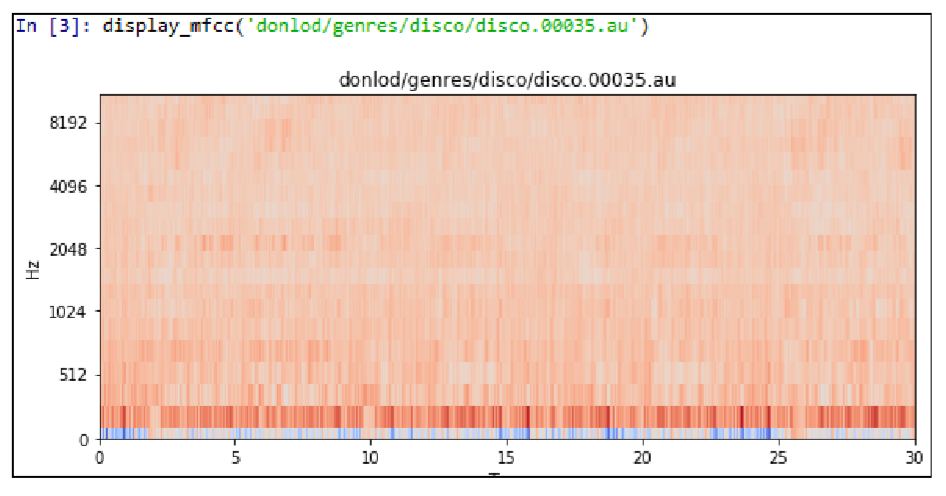
\includegraphics[width=4cm]{figures/1174040/chapter6/1.png}
                \centering
                  \caption{Hasil dari Code Program display\_mfcc}
            \end{figure}
            
            \item Penjelasan Code Program extract\_feature\_song
            
            \lstinputlisting[firstline=27, lastline=36]{src/1174040/chapter6/1174040.py}
            
            \subitem Pada Code Program diatas akan menjelaskan tentang ekstrasi data feature dari lagu yang akan di olah. dengan menggunakan Variable Y yang berisi method LOAD dengan record datanya dari class F pada extract\_feature\_song lalu membuat Variable mfcc dengan nilai yang akan meload data mfcc dari class Y, lalu melakukan normalisasi pada data Variable mfcc dengan penggunaan np.amax dengan nilai np.absolute(mfcc) lalu melakukan return dengan method np.ndarray.flatten(mfcc)[:25000] dimana data yang akan dibaca adalah sebanyak 25000 data dengan nilainya adalah array.
            
            \begin{figure}[H]
                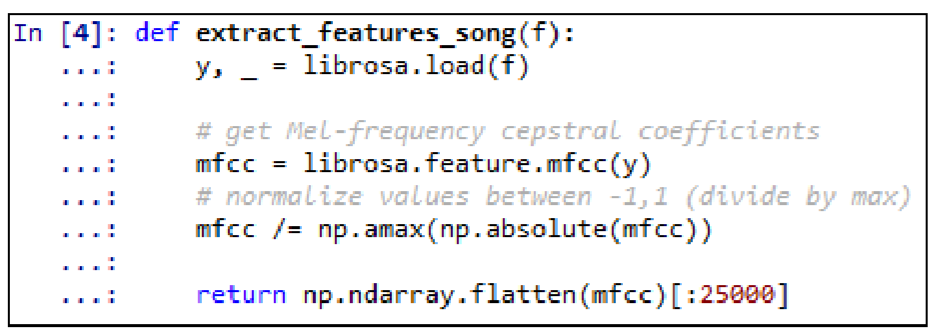
\includegraphics[width=4cm]{figures/1174040/chapter6/2.png}
                \centering
                  \caption{Code Program extract\_feature\_song}
            \end{figure}
            
            
            \item Penjelasan Code program  generate\_features\_and\_labels
            
            \lstinputlisting[firstline=38, lastline=56]{src/1174040/chapter6/1174040.py}
            
            \subitem pada code ini dimulai dengan membuat 3 data Variable array dengan format 2 nilai kosong dan 1 memiliki nilai. dimana data tersebut akan diolah dengan perintah FOR untuk membagi datasetnya sesuai dengan data GENRE yang telah ada. dengan menggunakan NUMPY pada perintah selanjutnya untuk melakukan pembagian data dan dikonversikan menjadi data one-hot encoding.
            
            \subitem hasil dari penggunaan perintah generate\_features\_and\_labels dapat dilihat pada gambar
            
            \begin{figure}[H]
                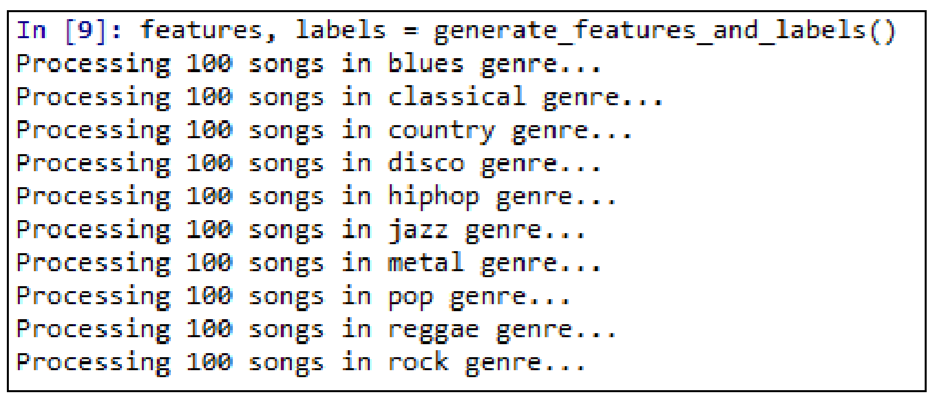
\includegraphics[width=4cm]{figures/1174040/chapter6/3.png}
                \centering
                  \caption{Code Program generate\_features\_and\_labels}
            \end{figure}
            
            \item Penjelasan tentang Kenapa proses pada generate\_features\_and\_labels lama
            
            \lstinputlisting[firstline=58, lastline=59]{src/1174040/chapter6/1174040.py}
            
            \subitem pada bagian penampilan hasil tersebut bisa lama dikarenakan data yang diolah itu tidaklah sedikit yang artinya memiliki data yang banyak, dimana masing - masing data yang diolah akan dilakukan cek terlebih dahulu untuk menentukan GENRE yang sesuai dan data tersebut akan dibagi menjadi 100 data yang telah dikonversikan menjadi data one-hot encoding.
            
            \item Penjelasan tentang pembagian data training sebesar 80 persen.
            
            \lstinputlisting[firstline=65, lastline=66]{src/1174040/chapter6/1174040.py}
            
            \subitem pemisahan data tersebut adalah untuk memastikan bahwa sistem telah siap untuk dilakukan uji coba dengan benar, dimana sistem tersebut telah dilakukan test dengan menggunakan testing data sehingga data yang akan didapatkan nanti dari penggunaan training data tidaklah terlalu jauh untuk nilai akhirnya. hasil dari penggunaan training\_split dapat dilihat pada gambar 
            
            \begin{figure}[H]
                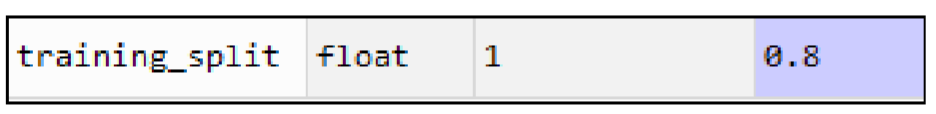
\includegraphics[width=4cm]{figures/1174040/chapter6/4.png}
                \centering
                  \caption{Hasil Code Program training\_split}
            \end{figure}
            
            \subitem dan berikut ini adalah hasil akhir dari data yang telah dipisahkan menjadi data TEST dan TRAIN dengan data tersebut sudah dilakukan SHUFFLE (acak) terdapat pada gambar.
            
            \begin{figure}[H]
                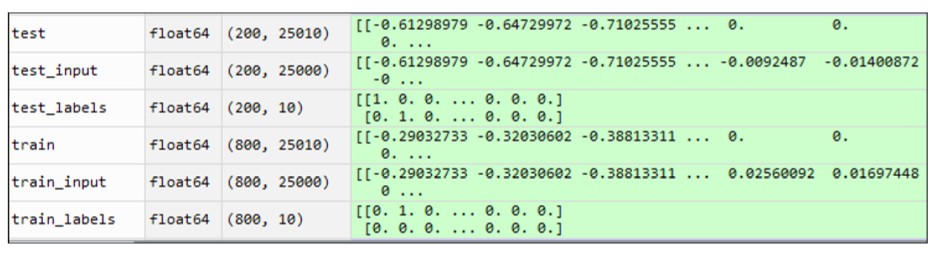
\includegraphics[width=4cm]{figures/1174040/chapter6/5.png}
                \centering
                  \caption{Hasil Code Program training\_split}
            \end{figure}
            
            \item Penjelasan parameter fungsi Sequential
            
            \lstinputlisting[firstline=92, lastline=98]{src/1174040/chapter6/1174040.py}
            
            \subitem fungsi Sequential pada code program ini adalah untuk mengolah data inputan agar sesuai dengan fungsi - fungsi yang ada pada code tersebut, dimana data yang akan diolah akan dilakukan pembentukan terlebih dahulu dengan menggunakan perintah pada Library NUMPY yaitu SHAPE dengan data yang digunakan adalah train\_input.
            
            \subitem pada gambar dibawah ini adalah keluaran dari RUNNING code tersebut
            
            \begin{figure}[H]
                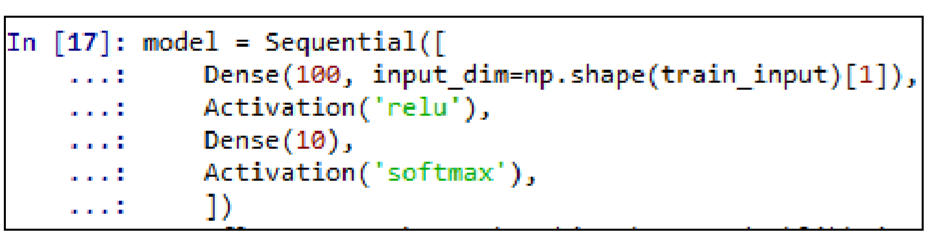
\includegraphics[width=4cm]{figures/1174040/chapter6/6.png}
                \centering
                  \caption{Hasil Code fungsi Sequential}
            \end{figure}
            
            \item Penjelasan parameter fungsi Compile
            
            \lstinputlisting[firstline=100, lastline=103]{src/1174040/chapter6/1174040.py}
            
            \subitem fungsi Compile digunakan untuk melakukan proses yang akan mengecek data parameter yang akan digunakan dari data yang telah diolah dari proses Sequential. hasil dari RUNNING pada fungsi Compile dapat dilihat pada gambar
            
            \begin{figure}[H]
                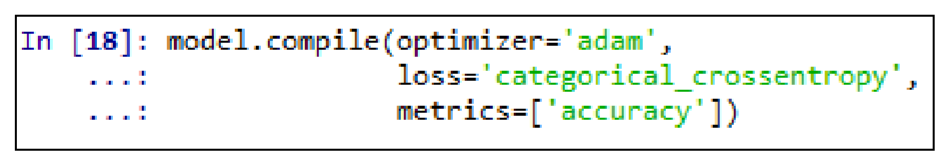
\includegraphics[width=4cm]{figures/1174040/chapter6/7.png}
                \centering
                  \caption{Hasil Code fungsi Compile}
            \end{figure}
            
            \subitem pada gambar dibawah ini adalah hasil dari penjelasan tentang data Sequential dan Compile
            
            \begin{figure}[H]
                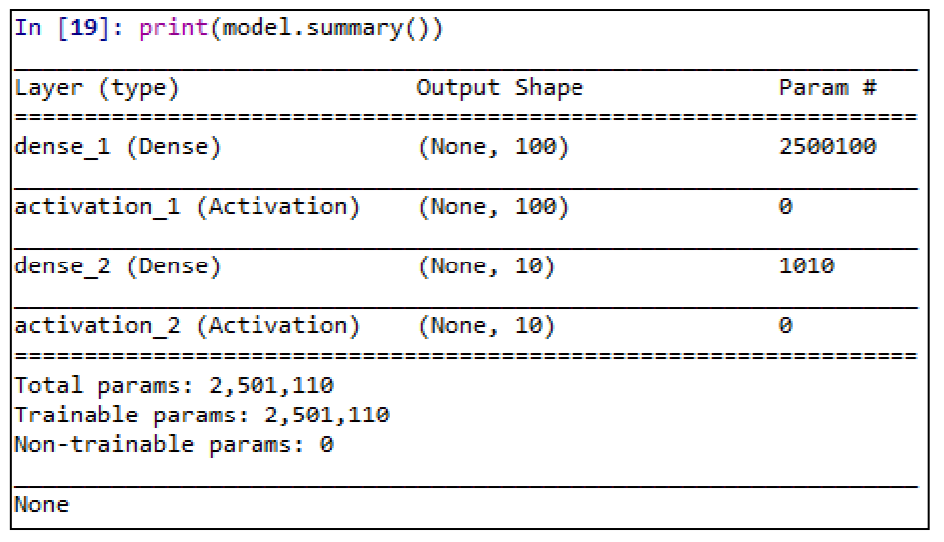
\includegraphics[width=4cm]{figures/1174040/chapter6/8.png}
                \centering
                  \caption{Hasil Code Program Summary}
            \end{figure}
            
            \item Penjelasan parameter fungsi Fit
            
            \lstinputlisting[firstline=107, lastline=109]{src/1174040/chapter6/1174040.py}
            
            \subitem fungsi Fit digunakan untuk mengolah data dari 10 label data menjadi 10 File datasets, yang kemudian akan dihitung untuk mengukur tingkat akurasi penilaiannya untuk keakuratan data yang diolah serta tingkat Loss (gagal) data yang terjadi. hasil dari RUNNING fungsi Fit dapat dilihat pada gambar.
            
            \begin{figure}[H]
                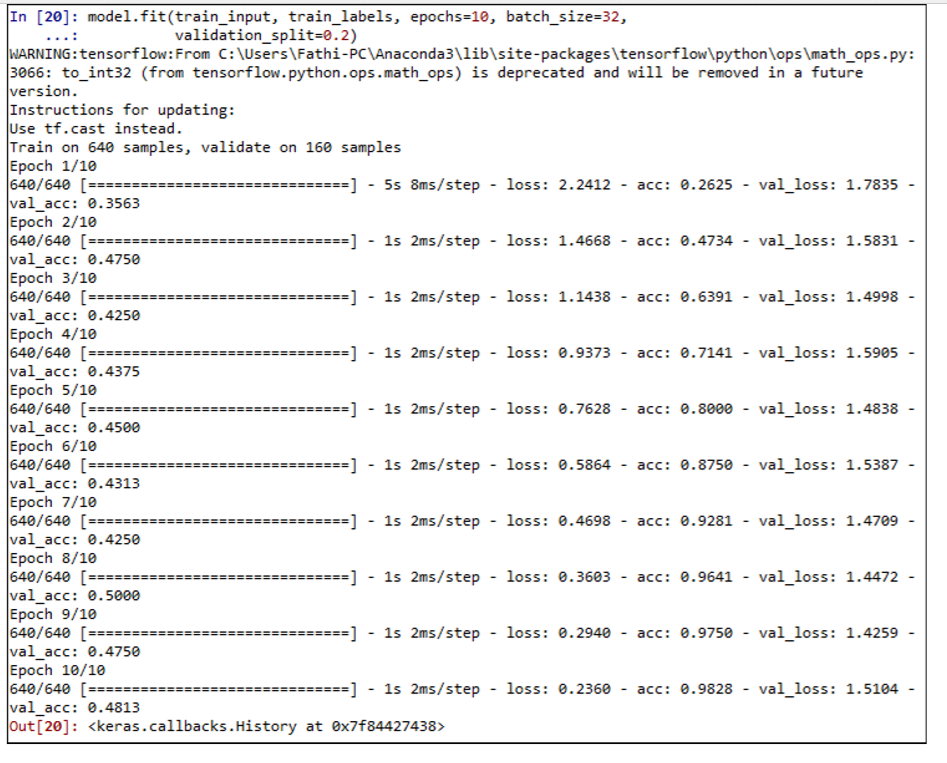
\includegraphics[width=4cm]{figures/1174040/chapter6/9.png}
                \centering
                  \caption{Hasil Code fungsi Fit}
            \end{figure}
            
            \item Penjelasan parameter fungsi Evaluate
            
            \lstinputlisting[firstline=111, lastline=112]{src/1174040/chapter6/1174040.py}
            
            \subitem fungsi Evaluate digunakan untuk mengevaluasi data yang telah diolah dengan menggunakan perintah fungsi Seqeuntial, Compile dan juga Fit. untuk hasilnya dapat dilihat pada gambar.
            
            \begin{figure}[H]
                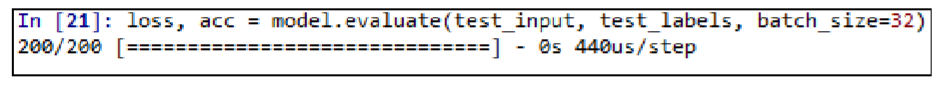
\includegraphics[width=4cm]{figures/1174040/chapter6/10.png}
                \centering
                  \caption{Hasil Code fungsi Evaluate}
            \end{figure}
            
            
            \lstinputlisting[firstline=114, lastline=116]{src/1174040/chapter6/1174040.py}
            
            \subitem untuk data yang ditampilkan pada gambar dibawah ini adalah data yang telah disusun untuk membandingkan tingkat Akurasi dan Loss yang terjadi.
            
            \begin{figure}[H]
                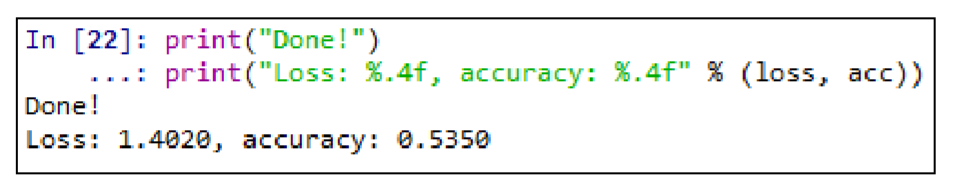
\includegraphics[width=4cm]{figures/1174040/chapter6/11.png}
                \centering
                  \caption{Hasil Code fungsi Evaluate}
            \end{figure}
            
            \item Penjelasan parameter fungsi Predict
            
            \lstinputlisting[firstline=118, lastline=119]{src/1174040/chapter6/1174040.py}
            
            \subitem fungsi Predict adalah untuk membandingkan tingkat Akurasi dari data pada setiap label yang ada pada dataset GENRE dimana data akurasi nilainya yang tertinggi maka akan diambil sebagai hasil akhir untuk nilai akurasi Predict. hasil RUNNING dapat dilihat pada gambar
            
            \begin{figure}[H]
                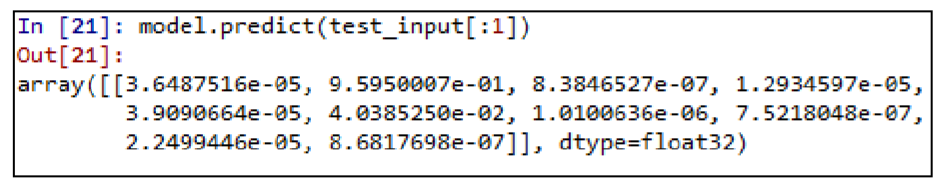
\includegraphics[width=4cm]{figures/1174040/chapter6/12.png}
                \centering
                  \caption{Hasil Code fungsi Predict}
            \end{figure}
            \end{enumerate}